\documentclass{cmspaper}
\def\RCS$#1: #2 ${\expandafter\def\csname RCS#1\endcsname{#2}}
\RCS$Revision: 1.3 $
\RCS$Date: 2004/05/27 12:46:29 $

\usepackage{graphicx}

\begin{document}
\begin{titlepage}
  %\whitepaper 
  \internalnote{2004/XXX} % \cmsnote{2005/000} % \conferencereport{2005/000}
  \date{Revision \RCSRevision, \RCSDate}
  \title{Software agents in data and workflow management during DC04- post-mortem}

  \begin{Authlist}
  \end{Authlist}

  %\Instfoot{cern}{CERN, Geneva, Switzerland}
  %\Anotfoot{a}{On leave from prison}
  %\collaboration{CMS collaboration}

  \begin{abstract}
	This paper collates the experience gained in data distribution during
	DC04. It details the structure used, and discusses the overall behaviour
	of each of the components.
  \end{abstract} 

  %\conference{Presented at {\it Physics Rumours}, Coconut Island, April 1, 2005}
  %\submitted{Submitted to {\it Physics Rumours}}
  \note{Preliminary DRAFT version}
\end{titlepage}

\setcounter{page}{2}

\section{Introduction}
During the March and April 2004 CMS undertook a large scale data
challenge (DC04) with the goal of sustained data distribution over an
extended period, with data streaming from the T0 as if from the CMS
detector running at 25\% of startup luminosity (25 Hz, or events per
second).

In the preparations for DC04 it became apparent that the LCG tools
available did not fully meet the requirements of the experiment. Grid
projects had developed useful APIs to meet certain needs- e.g. for
point-to-point file transfer using gsiFTP \cite{rmapi}; to mirror data
between sites \cite{gdmp}; or to maintain a catalogue of files
\cite{rls}. However, the tools were coupled together to form a replica
management system that did not meet overall experiment requirements
for data transfer during DC04: namely, that transfer should be
scheduled and directed in a large-scale manner, at dataset
granularity, rather than in a point-to-point opportunistic manner at
file granularity.

A significant part of DC04 preparation and running was therefore the
design and development of a working directed replica management system
for CMS. This paper outlines the experience gained in designing,
developing and using the system. It does not examine the apparent
mismatch between requirements published and received between the
experiment and Grid developers.

CMS developed a system that to meet the following requirements of
DC04 \cite{dc04plan}:
\begin{list}{}{}
\item Data streams from the T0 as if from the CMS detector running at 25Hz.
\item Datasets will be allocated and delivered to certain T1s.
\item The system must manage the propagation fo files to the T1s automatically.
\item The system must be scalable (requiring a minimum of supervision and intervention).
\end{list}

The system designed was based on a structure of semi-autonomous
software agents collaborating by sharing information in a global
space. It was was rapidly prototyped and put into production during
the months of February and March 2004.

The system proved able to transfer 25 Hz reconstructed data, and to
reach sustained aggregate data rates of 30+ MBps. The system was also
used to analyse data in ``real time'' exhibiting a median latency of
only 20 minutes between files being ready for distribution and the
analysis results being available at a Tier 1.

\section{The data distribution system}
The CMS data distribution system for DC04 was a dataset management
structure, drawing on aspects of blackboard and multi-agent system
design \cite{FG96,C03,Setal03}. Persistent, stateful agents were
deployed at a number of geographically distributed sites, and handled
point to point propagation of files through the system. Communication
between agents (typically via messages announcing the presence of
files at some point in the system) was limited by design; propagation
of information through the agent system required the agents to post
information at a central ``blackboard''. This blackboard was
implemented in Oracle and named the Transfer Management Database, or
TMDB.

This architecture enabled us to maintain a coherent picture of system
state in a central location, making it relatively easy to diagnose and
solve problems. It also meant that agent development was characterised
by short timescales and simplicity.

Agent development was simple because the exchange of messages was used
to define the behaviour of a small range of agents, which could then
be implemented in a way that suited local developer groups. By doing
this any need for local functionality were easily met by implementing
a new agent, in whatever language was suitable. Strictly defined
message passing encouraged the localisation of complex functionality
within single agents \cite{B03}.

\subsection{Components and data flow}
The system comprised a data source (the Reconstruction farm at CERN),
a common transfer/state database (TMDB) and a hierarchy of agents that
managed and distributed the data. Other components- like a web front
end to manage the TMDB and monitor the status of the disk buffer from
which files are distributed- were developed as required.

The distribution system drew files from Castor stage disk and streamed
them to a number of T1s via export buffers dedicated to a specific
transfer mechanism. At the T1s the data were placed in mass storage,
and in some cases data was directed to T2s. The transfer of data
through the system was handled by a series of agents of limited
responsibility.

Files were placed in the Castor stage area by Reconstruction jobs. To
trigger distribution an XML catalogue fragment and checksum file were
placed in a dropbox- a disk folder- for an agent to find. These agents
then published file information in the RLS and the TMDB
(fig. \ref{fig:flow1}).

A Configuration agent at the T0 allocated files to specific T1s,
acting as a simple replica manager. Export Buffer agents (dedicated to
a number of T1s, all using the same distribution tool) scanned the
TMDB for newly allocated files. Generically, they drew these files
from the Castor stage area and placed them on an Export Buffer
(fig. \ref{fig:flow2}).

At each T1 an agent scanned the TMDB looking for files that were newly
available on the Export Buffer. It transferred these files to the
T1. Further agents ensured that the files were placed in mass
storage. As files appeared at T1s, other agents submitted the files to
analysis and published the results. In some cases, further agents
replicated files to T2 sites for analysis (fig. \ref{fig:flow3}).

\begin{figure}[tbp]
\centering 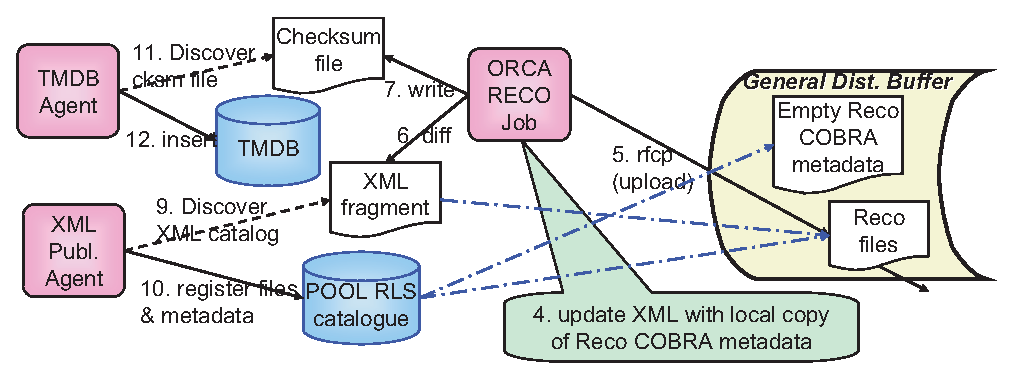
\includegraphics[angle = 90]{T0-flow.eps}
\label{fig:flow1}
\caption{Making data available to distribution during DC04.}
\end{figure}

\begin{figure}[tbp]
\centering
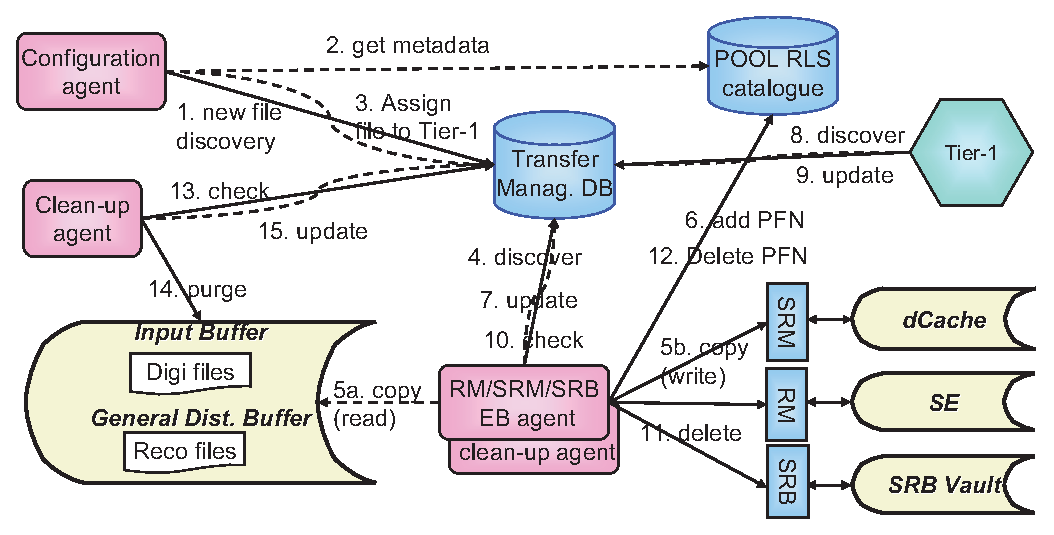
\includegraphics[angle = 90]{T0-flow-2.eps} 
\label{fig:flow2}
\caption{Insertion of data into distribution chains during DC04.}
\end{figure}

\begin{figure}[tbp]
\centering
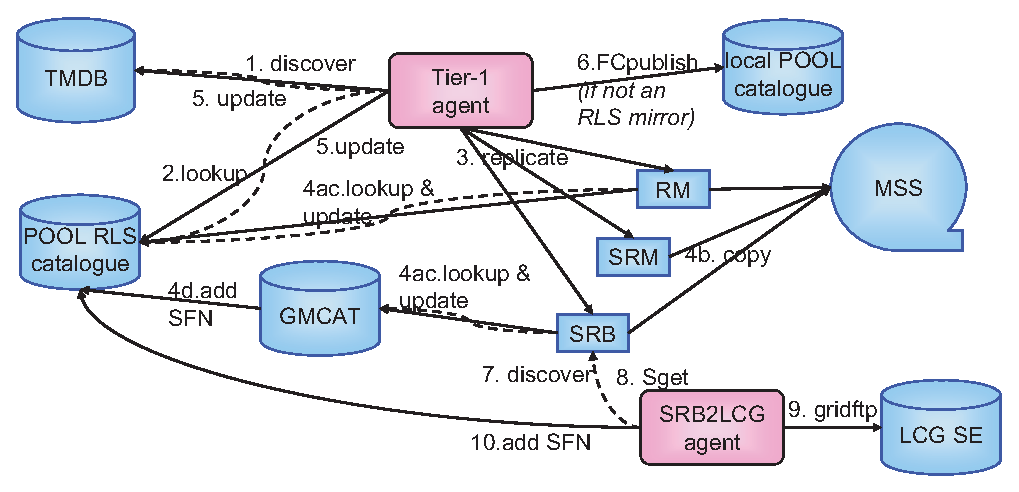
\includegraphics[angle = 90]{T1-flow.eps} 
\label{fig:flow3}
\caption{Transfer of files to T1 mass storage during DC04}
\end{figure}

\subsection{DC04 distribution infrastructure}
During DC04 data was distributed via three ``chains'', corresponding
to three flavours of distribution middleware. These middleware tools
were the LHC Computing Grid (LCG) \cite{lcg}, the Storage Resource
Manager (SRM) \cite{srm} with dCache \cite{dcache} and SRB \cite{srb}
(fig. \ref{fig:chains}).

\begin{figure}[tbp]
\centering
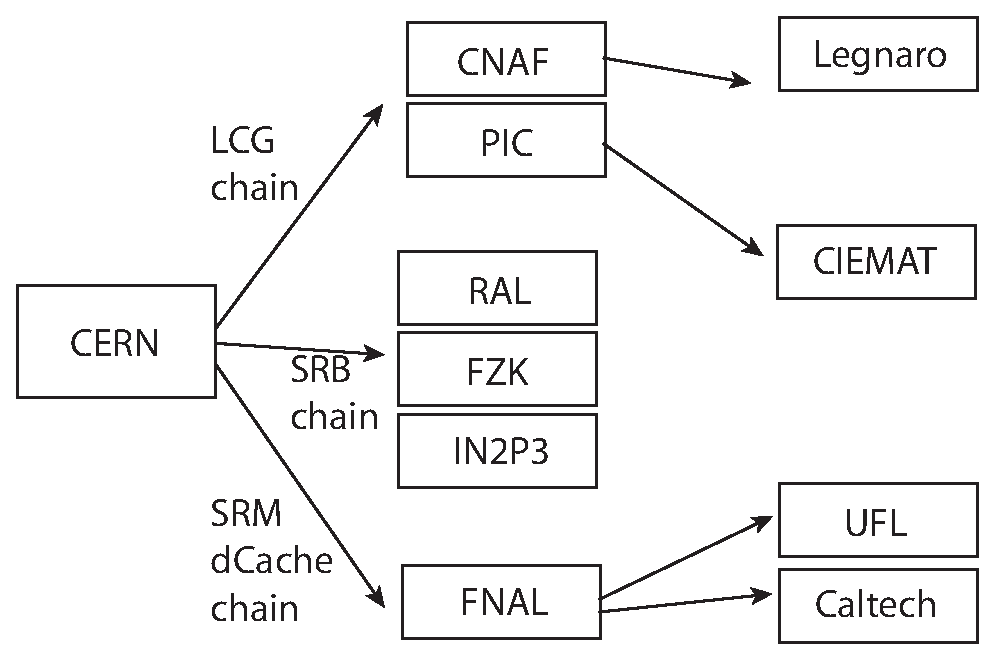
\includegraphics[width=15cm, angle = 90]{chains.eps} 
\label{fig:chains}
\caption{Overall view of the distribution chains deployed during DC04.}
\end{figure}

The LCG chain used LCG Replica Manager Java command line tools
\cite{rmapi} and Globus globus-url-copy \cite{globus} to make
transfers using gsiFTP \cite{gsiftp}, and the Local Replica Catalogue
C++ API \cite{rmapi} to query the RLS and make updates. The chain
deployed two varieties of LCG Storage Elements (SEs) as file buffers:
an LCG "classic", or disk only, SE; and an LCG Castor SE with a
stager-managed disk pool with access to tape.

All chains used the LCG Replica Location Service (RLS: \cite{rls}) as
a repository of filename and metadata information. For future
reference, the RLS deployed during DC04 comprised a single Local
Replica Catalogue and Replica Metadata Catalogue deployed at CERN. The
distribution chains used LCG tools- either LRC tools or POOL
\cite{POOL} File Catalog tools- to query and make entries in the
catalogue. Local POOL file catalogues were also deployed as a means of
accessing file information for analysis jobs at the T1s and T2s.

SRM is an acronym denoting the Storage Resource Management interface,
which provides generic access to any storage resource
\cite{srm}. Superficially SRM provides a defined two step interaction
through which a file can be obtained from any storage medium for which
the user has a Storage URL (SURL), which contains the hostname of the
medium. During an SRM transaction the client presents an SRM server
with the SURL, is is returned a Transport URL (TURL) which indicates
the current (possibly temporary) location of the file and a transport
protocol that can be used to access it. dCache disk buffers were
deployed to form the SRM chain infrastructure, and gsiFTP used to make
transfers; dCache \cite{dcache} is a disk pool and tape storage
management software as file buffers.

SRB is an acronym for the Storage Resource Broker, another middleware
that presents a uniform generic interface to storage media
\cite{srb}. SRB differs from the SRM and LCG in that it presents a
uniform global interface to the user; that is, a user is typically
unaware of where a file within SRB physically resides. SRB filespace
and file metadata is stored within a metadata catalogue named the
MCat. SRB vaults were deployed as file buffers to form the SRB chain,
and used Sput and Sreplicate commands to transfer files. The SRB and
LCG file catalogues were syncronised by a standalone application named
GMCat.

More detailed descriptions of each chain, and related experience with
it during DC04, can be found below.

\section{Experience}
Development was rapid, and mostly straightforward. Several versions of
export buffer, T1 transfer and mass storage agents were implemented
within several weeks of the first examples being made available. This
rapid development was due in part to the extremely limited
responsibility of each agent, and the easy breakdown of agent workflow
into chunks of functionality like ``publish state in database'',
``check for new guids'' (defined by TMDB interactions).

Agents were implemented in a variety of languages: at first, a
scripting approach was taken, and agents were implemented in Perl and
Bash scripts. The agents relied on command line tools to access the
Oracle TMDB and POOL File Catalogues, and to make file
transfers. Experience during DC04 modified this approach, and agents
implemented in lower level languages (C++) appeared.

Command line tools proved to be too generic to support intensive bulk
use, meaning that agent developers moved naturally to using the
underlying component APIs to effectively write their own focused
distribution tools. However, the existence of these command line tools
enabled the rapid initial prototyping of agents using scripting
agents.

Each chain of agents was coded and trivially tested within six weeks,
and developed and tested over the whole of DC04 (eight weeks).

It was found that the collaborative approach- sharing information
between agents on a blackboard- enabled the development of new agents
with functionality that was not foreseen. By way of example, a
cleaning agent was implemented at the T0 to manage Castor stage
space. It required a somewhat more sophisticated strategy than just
checking whether files were safe at MSS before migrating them to
tape. Instead, using information already in the TMDB, it was able to
rank files and thereby efficiently prioritise them for migration.

This sort of evolution was not without difficulty- the original design
of the TMDB meant that adding new information schema to the database
was somewhat costly. It is however something that can easily be
overcome in future versions of the database (see below).

Coordination and management of people and agents proved inefficient,
and it became clear that global mechanisms for suspending, restarting
and monitoring agents needed to be deployed in future versions. During
DC04, almost all system shutdown/restarts required an email sent to
each operator, with the action only taken when all replies were
received. In a similar vein, the presentation of global system state
must be improved: during DC04 a limited amount of all information was
available via a simple web page. In the future some interpretive
interface must be created to highlight current problems and warnings,
and reveal more sophisticated information (file transfer rates, etc)
in a more immediately intuitive and useful way.

\subsection{Overall behaviour}
A total of 564,273 files were placed in distribution during DC04. At
the end of DC04 there were 1,969,976 replicas being actively managed;
a total of 2,942,368 single replica chains were known \footnote{Here a
replica chain implies a single entry per set of replicas from source
to destination; e.g. from castor to RAL MSS. The number of replcias
involved in such a chain might be 4 times larger than this number, so
the system was aware of somewhere between 2,942,368 and 11,769,472
replicas in total.}.

A total of 278,081 files were made safe on tape, with the following
breakdown: 33\% IN2P3, 32\% PIC, 28\% RAL, 8\% INFN, 0\% FNAL, 0\%
FZK.

One might use the lifetime of files in the system as a useful metric
for measuring system performance, defining the lifetime of files as
the period between appearance and migration to Castor at
CERN. However, there were two significant barriers to efficient
migration of files at CERN. First, the mechanism for migrating to
Castor at CERN was only implemented late in DC04. Second migration was
hampered by technical issues with the SRB chain which meant that a
large backlog of files was generated. Studying the comparison of
lifetime with time of appearance, it is clear that files that appeared
early remained in distribution for a long time, while files that
appeared late had a correspondingly shorter lifetime; the information
gained from such a study is negligible.

It is more meaningful to ask how long it was before files were
available for analysis at a T1: figures for this vary from
distribution chain to distribution chain, with the LCG chain to CNAF
taking between 10 minutes and a day and a half, and the LCG chain to
PIC taking only 20 minutes consistently (fig. \ref{fig:PIC-RTA}). More
detailed information on real time analysis during DC04 is available
elsewhere \cite{rtadoc}.

\begin{figure}[tbp]
\centering
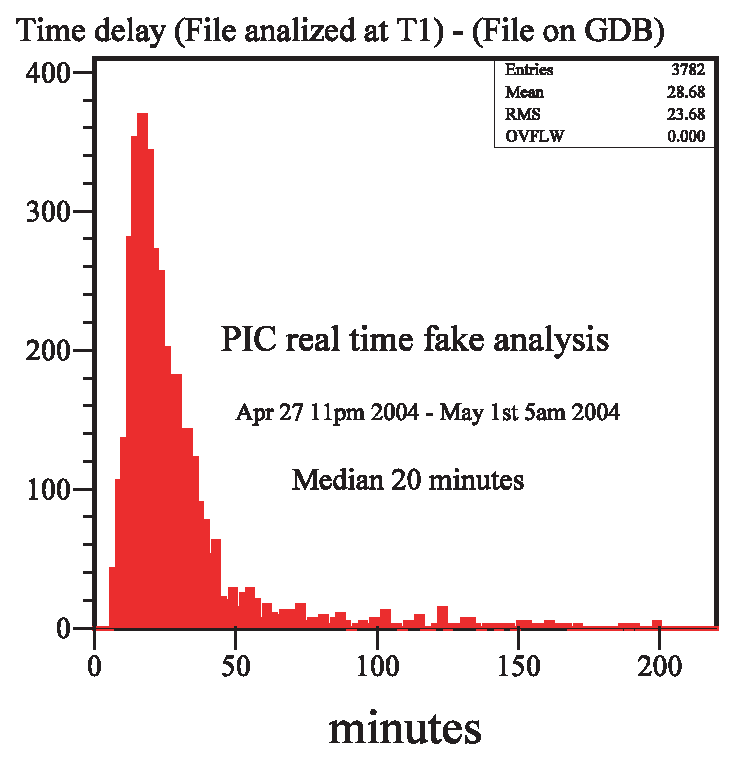
\includegraphics[width=10cm]{PIC-RTA.eps}
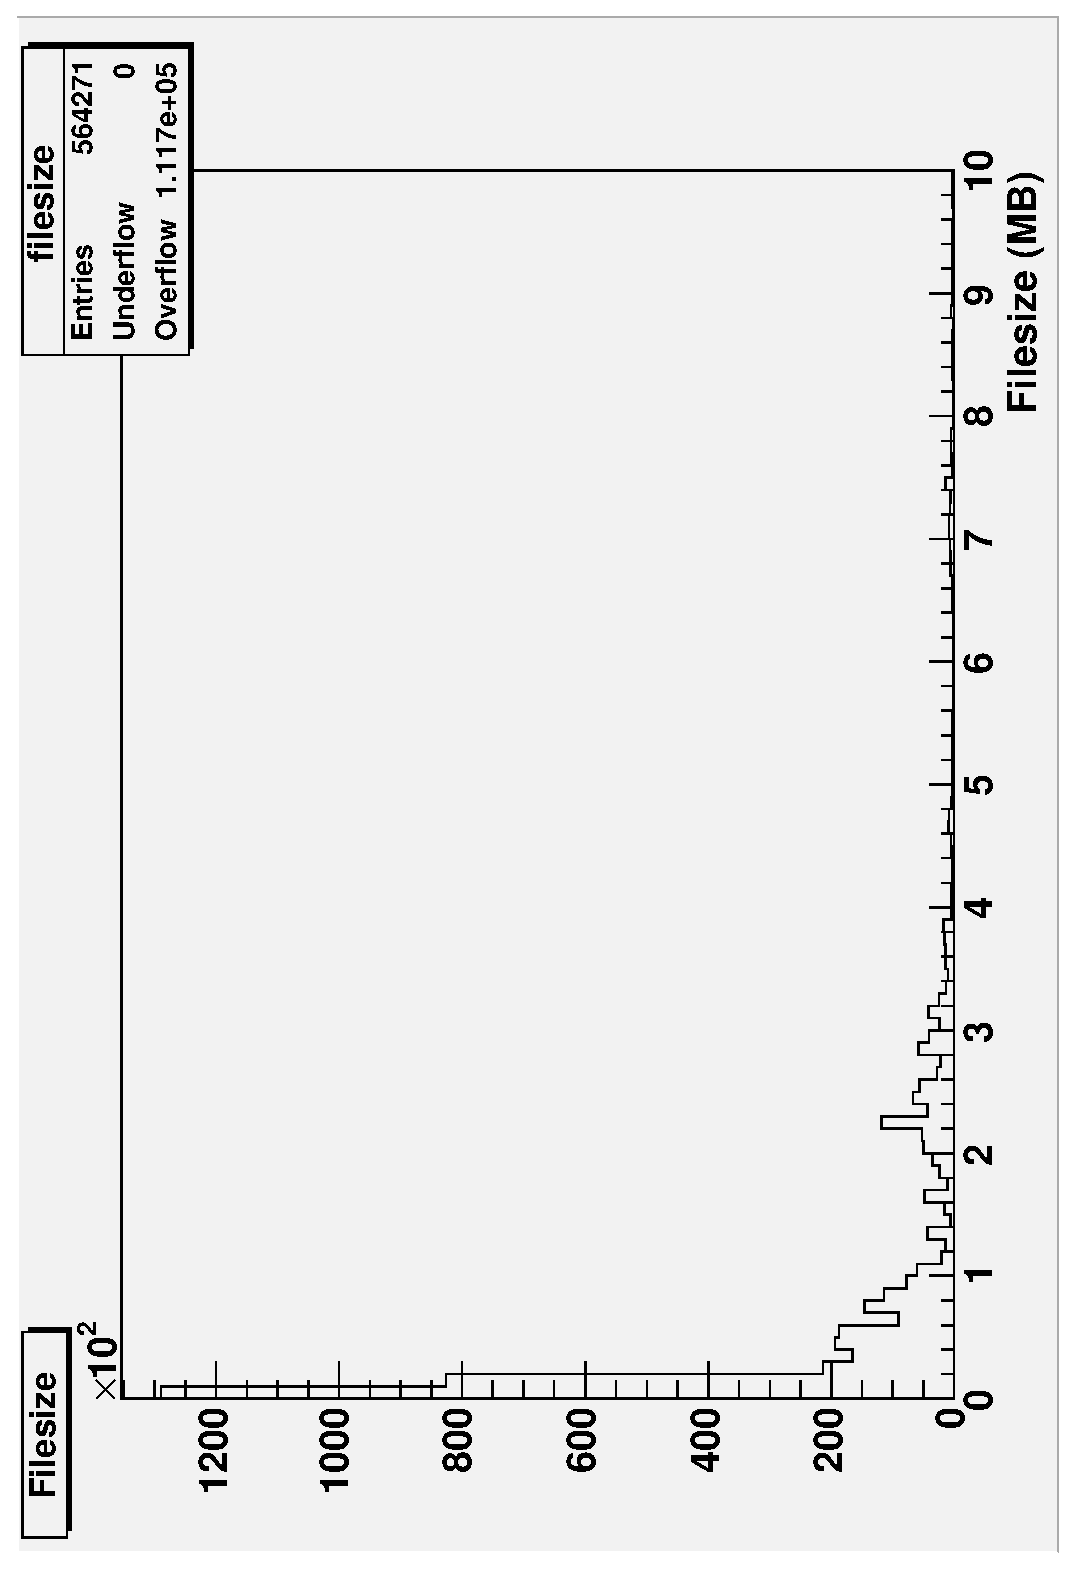
\includegraphics[width=10cm, angle=-90]{filesizes.eps}
\label{fig:PIC-RTA}
\caption{Upper:During the last four days of DC04 PIC were able to implement
a real time analysis system based on CNAF's system. Turnaround time
for analysis at PIC was much shorter and more consistent than CNAF at
a median of 20 minutes. Lower: Median filesize during DC04 was ~500 KB.}
\end{figure} 

Transfer rates varied greatly, and are treated in more detail
below. Generally however, transfer rates at the start of DC04 were
low- individual transfers reached maybe a MBps, with aggregate rates
pushing 10MBps. These low transfer rates were due to the small size of
files being pushed through the system. This is an example of poor
initial coupling between the data source and the distribution
system. Here the coupling is described as poor because it is easy for
reconstruction to produce small files, but difficult for distribution
to distribute them due to the overheads associated with each file,
independent in most cases of size. These overheads include catalogue
registration (which takes the same time despite file size); startup
times for Java Virtual Machines; and inefficient ramping of TCP/IP
window sizes for small file sizes.

During DC04 this poor coupling was mostly dealt with by working around
it. For example, poor transfer speeds were remedied by making as many
parallel transfers as possible; file and metadata catalogue accesses
were limited as far as possible; and the use of Java command line
tools was replaced by the use of C++ APIs.

At the very end of DC04 this poor coupling was improved to some extent
by the implementation of a "merging" step (detailed below) which added
files to one of a series of queues which expired and were written
after either a certain aggregate size or time limit was reached. File
sizes were typically ~500k median at the start of DC04
(fig. \ref{fig:PIC-RTA}).

Agent uptime was not monitored directly, and is difficult to
estimate. Some agent types would not publish themselves as
``available'' if they could not complete any file transfers- as
happened for example several times when the load on Castor was
high. Typically the agents implemented as Bash scripts suffered this
problem- the C agents were implemented in a slightly different way.
Interpretation of information about agent uptime is therefore
difficult to interpret from DC04 logs, an area for improvement in
future versions of the distribution system.

Due to bugs in the reconstruction code large numbers of files were
deemed of limited use for analysis. It was decided that these files
should be marked as bad, and removed from distribution. To do this a
new set of states indexed 90 and above was introduced. As agents
weren't looking for files in those states the files were never
transferred. The system therefore proved flexible enough to meet new
requirements during development.

\subsection{The TMDB}
In contrast to other databases used, the TMDB proved to be remarkably
stable, only experiencing a critical problem when log entries exceeded
the initial tablespace allocated.

Development of the TMDB continued throughout DC04 as new use cases
were discovered. The management of changes to the databases provided
useful experience for the future. Most changes were easily accomodated
thanks to a carefully designed database schema (for example, the
addition of new agents was handled gracefully)
(fig. \ref{fig:schema}).

\begin{figure}[tbp]
\centering
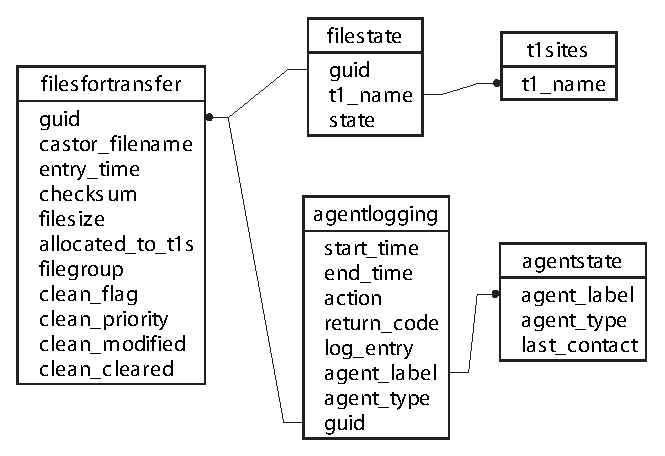
\includegraphics{v1_tmdb.eps}
\label{fig:schema}
\caption{The Transfer Management Database schema deployed during DC04.}
\end{figure} 

However, some changes- notably the addition of some forms of metadata
to the list of files for transfer- caused significant slow down in
access. During DC04 it became apparent that some specific metadata- an
entry denoting the filegroup, and some indication of cleaning
priority- was required. Adding this new metadata was seen as a ``one
off'', and was implemented as new fields in an existing table. At that
stage, however, the TMDB had several hundred thousand files registered
in it. The addition of new fields and entries to the database took
many hours, and impaired access for the agents.

Future versions of the TMDB will require that metadata be stored in a
separate table, thus avoiding this problem by allowing the addition of
metadata in key:value pairs.

The discussion of which metadata to add to the database- from LFNs
through replica to application metadata- continued throughout
DC04. Addition of metadata to the TMDB was vigorously opposed to avoid
it being seen as a permanent repository of metadata (in principle all
information in the TMDB is transient). It became apparent that the
ability to add metadata to replica entries- even changing the schema
of metadata, or having a varying schema for each replica- was
essential, especially during development.

\subsection{The DC04 Replica Location System (RLS)}
The LCG-2 RLS was deployed as a global service for lfn:guid:pfn and
metadata lookups during DC04: a Local Replica Catalogue (LRC) and
Replica Metadata Catalogue (RMC) were deployed on a Sun cluster at
CERN running Oracle; the RLS web service frontend was deployed using
Oracle Application Server. CMS' DC04 was the first full-scale test of
the RLS.

These catalogues were accessed in a variety of ways- for example,
using the LRC C++ API for direct access to the LRC, or through POOL
File Catalogue tools (the LRC-RMC combination can be represented as a
single POOL File Catalogue).

The RLS proved to be a critical component during DC04, even if only
judged on the number of processes accessing it (table
\ref{table:rls}).

\begin{table}
\begin{tabular}[tbp]{|l|l|l|}
\hline User & Use of RLS & Tool
\\ \hline Publishing Agent & Registration on appearance & FCpublish
\\ Configuration Agent & Query the RLS metadata & FClistMeta
\\ Export Buffer Agents & Register new mappings & FCaddReplica
\\ & & C++ LRC API
\\ GMCat & Maintain SRB : LRC filespace mappings & LRC java API
\\ Tier-1 Agents & Register new mappings & FCaddReplica,FCpublish
\\ & Publish sub-RLS into local MySQL POOL catalogue & C++ LRC-API
\\ LCG Analysis jobs & Through Resource Broker & Replica Manager
\\ & Register the private output data & 
\\ Humans & diagnosing problems & FC commands
\\ \hline
\end{tabular}
\label{table:rls}
\caption{Summary of the many uses of the RLS during DC04. FC* commands are those provided by POOL.}
\end{table}

The RLS at CERN was found to be a critical bottleneck early in the
challenge, and a significant amount of effort was expended in
developing it so that performance was brought close to
requirements. Even at the end of DC04 however it was still not being
used as a complete global catalogue; MySQL POOL catalogues that
partially replicated information in the RLS were deployed to enable
analysis at the T1s and T2s. These catalogues were not fully
syncronised, although information was published to them from the RLS.

Problems with the RLS stemmed from the performance of the RMC, and the
implementation of the catalogue: the LRC and RMC are implemented as
separate databases, so a query based on metadata must look up
information in the RMC, and then correlate it with information in the
LRC, rather than using the database server to make the correlation for
the user.

In general inserting information into the LRC was slow, and using the
RMC was slower. Looking up file information by GUID met performance
requirements, but queries, including queries by GUID, took a long
time. Throughout DC04 discussions on performance were held with the
catalogue developers, and as a result a new optimized version was
released just after DC04.

Over one of the earliest busy periods of DC04- when the LRC and RMC
began to fail- there were around $10^6$ interactions with LRC Oracle
backend, and $3\times10^6$ interactions with the RMC per day.

In total $~570$k lfns were stored in the RLS during DC04, each with
5-10 pfns and 9 metadata attributes. Inserting information into RLS
was fast enough once appropriate tools were developed. For example,
registering a new mapping using the LRC C++ API took 0.1-0.2 s per
mapping, while using the POOL CLI with a GUID at a time took seconds
per mapping.

Inserting files with metadata into the RLS was slow in comparison,
although approximately usable at around 3 s per file. There were
periods, however, where intervention was required on the server and
insertion times dramatically reduced
(fig. \ref{fig:rls}). Interventions included cleaning of log
partitions, switching backend nodes, and optimizing queries.

\begin{figure}[tbp]
\centering
\includegraphics[width=10cm]{rls.eps}
\label{fig:rls}
\caption{The time taken to register all files in drops as they appeared at the end of Reconstruction jobs shows some variation, with periods of high data production associated with longer registration times (near the middle of the plot). Typically there were 16 files per drop.}
\end{figure} 

Querying information from RLS was in general very slow. Looking up
file information by GUID seemed sufficiently fast, but bulk queries by
GUID- strictly a metadata-based search- took seconds per file. Other
queries on metadata were too slow- for instance, querying for all
files of a specific ``owner'' took hours. In contrast, it took two
minutes to dump the entire catalogue to file after gaining access to
the Oracle backend.

The problem was also not POOL-related: for comparison, POOL MySQL or
XML catalogues dumps were a minimum factor 10 faster than an
equivalent dump from a POOL RLS catalogue. It is entirely possible
that a POOL MySQL catalogue could have met the demands of DC04:
however, some transfers were undertaken using LCG tools that required
an LCG RLS.

In summary, several workarounds or solutions were provided to speed up
the access to RLS during DC04: use of the Java Replica Manager CLI was
replaced by use of the C++ API; POOL developed improvements and
workarounds; and CERN IT were able to index some meta data attributes
in RLS (by default, none of the RLS tables are indexed). There were a
number of requirements that were not met at the start of DC04:
transactional access; a small overhead compared to to direct RDBMS
catalogues; and fast queries.

Each of these issues needs to be met if the RLS is to be used in the
future as the file catalogue of choice. Wheher it remains the ideal
solution to storing replica metadata also needs to be examined.

\subsection{Dropbox agents}
A series of agents at CERN handled the coupling between the
Reconstruction farm and the distribution system. Their design strategy
was somewhat different to the other agents: they did not communicate
as such, but rather functioned as limited file processors which
propagaetd files through a series of dropboxes, or local folders. By
doing this it was possible to implement a series of agents focused on
specific tasks (e.g. staging files to disk, or merging files) that
together formed a very powerful file state management tool.

The dropbox agents in existence at the end of DC04 undertook the
following series of tasks
\begin{list}{}{}
\item Publish COBRA META files.
\item Update local filenames in XML catalogue.
\item Pin files in Castor.
\item Publish XML catalogue to RLS.
\item Publish RLS entries for merged files.
\item Publish information in the TMDB.
\item Filter Zip files already processed.
\item Funnel files to a merging process.
\item Merge files into Zips.
\item Rank files on GDB for migration.
\item Migrate files to tape.
\end{list}
Typically they performed well, each taking \~0.01s per drop of O(10)
files, easily fast enough to keep pace with steady state production,
with some exceptions. The dropbox agents that interacted with the
RLStended to underperform, principally due to the lack of bulk
operation access to the RLS.

During DC04 realtime analysis required some mechanism by which it
could determine whether all the files of a given dataset had
arrived. This could be determined using ``filegroup'' metadata, where
filegroup was a unique key generated during reconstruction that could
be used to tie all files in a given dataset together. This metadata
was added to the filesfortransfer TMDB table, as discussed above.

One of the dropbox agents implemented the file merging step used in a
large file transfer stress tests at the end of DC04. Files were
assembled into larger chunks based on the data type.  Each such queue
had a user-configurable size and time limit.  When either limit
expired, the files collected were merged into a bigger file and sent
downstream.  Files were merged into uncompressed zip archives;
individual files in the archive retained their identity, and the rest
of the system continued to see them as individual files.  The only
difference between files in Zips and the files produced by Reco was a
non-standard URL such as ``zip-member:rfio:/.../foo.zip\#member-name''.
COBRA has means to read such ``sub-files'' directly, redirecting the
file access into a sub-byte-range inside the archive.

The merging process required significant processing power. Several
zip-making agents must be run in parallel because sometimes rfcp from
GDB takes so long that queues would stall- sometimes up to two hours.
Unfortunately maintaining several concurrent processes each reading
and writing 1.5GB data to disks is something Linux 2.4 kernels
apparently do not do very well. As a result the merging agents had to
be run on a dual processor Sun box with SAN disks. With this
infrastructure there were no problems keeping up with production or
processing backlogs from delays.


\subsection{SRM chain}
The SRM distribution chain comprised an SRM Export Buffer at CERN
providing access to a dCache disk pool, and an SRM import buffer at
FNAL providing access to Enstore, again via dCache.

At the T0, the SRM export buffer handled staging of files from Castor
to dCache disk pool, where they were pinned until transferred.

The transfer agent copied files from the export buffer to the T1
import buffer by initiating a third party SRM transaction to receive a
TURL from the export buffer, then using gridFTP to make the transfer.

The use of storage media that presents a uniform SRM interface to the
outside world is a model for the way storage will ideally behave in
future versions. Use of SRM throughout would enable us to create
generic transfer agents, and make implementing them simpler, as
operations like file staging, etc would be handled automatically
\footnote{Although whether the SRM method for handling staging is best
for us is not clear. If we only use SRM to handle this, then ideally
SRM gives the transfer agents a way to trigger a stage and return
simply and gracefully when necessary.}.

Initially problems were seen with repeated authentications: the agents
were developed so that multiple streams, with multiple files in each
stream, could be used to transfer files, reducing the number of
authentications required. Transfer rates of over 10 MBps could be
sustained for long periods (fig. \ref{fig:FNAL-network}).

\begin{figure}[tbp]
\centering
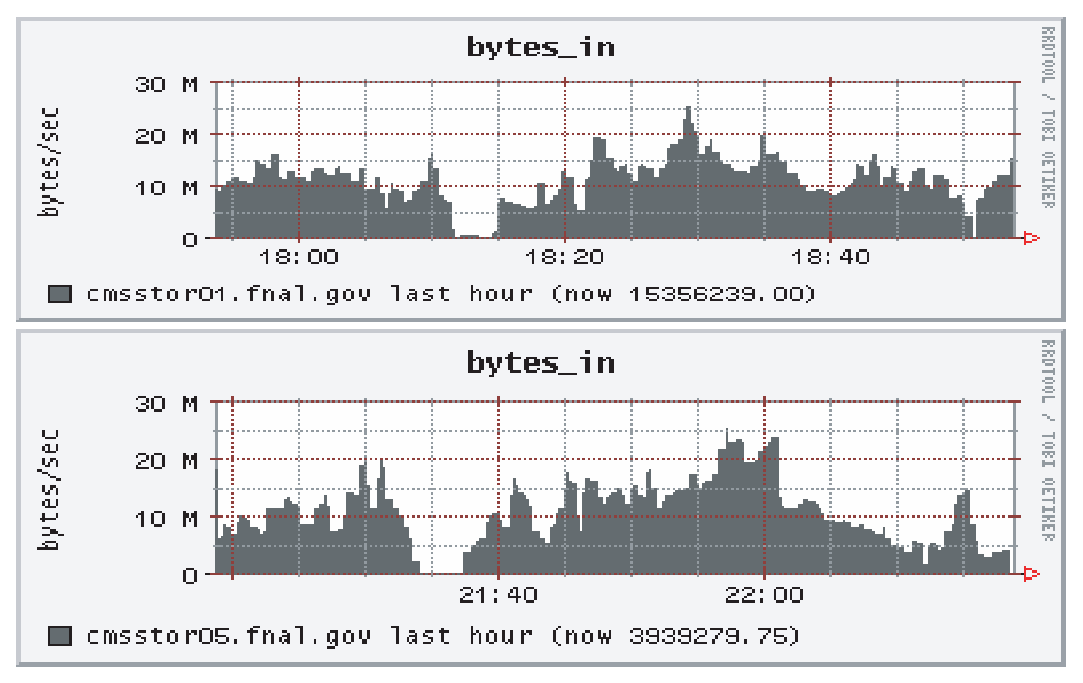
\includegraphics[width=10cm]{FNAL-network.eps}
\label{fig:FNAL-network}
\caption{The SRM chain was able to sustain transfer rates of more than 10 MBps into FNAL for long periods.}
\end{figure} 

In contrast to other techniques, the use of SRM eased agent
development with features like automatic directory creation, file
migration and staging, and automatic failure recovery. Similar
features were successfully implemented as parts of the distribution
system in, for example, the LCG chain.

However, during DC04 it proved difficult to install monitoring
technology, which meant that hardware failures had to be identified by
a human operator, and restarts handled manually. In common with other
distribution chains the SRM chain had difficulties with the large
number of small files, which necessitated an increase in the number of
tapes available and the deployment of a larger namespace service.

FNAL also deployed a MySQL POOL catalogue to enable access to the
transferred data in the US; they found its performance more than
adequate for the task. Initially the publishing of entries from the
RLS to the FNAL POOL catalogue proved difficult, with the RLS queries
taking a long time (see above). Close work between agent developers at
CERN and FNAL brought about a 100-fold increase in performance.

All data access at FNAL was attempted through dCache via a ROOT
plugin- so that COBRA based applciations could trivially access the
data. Read performance was shown to be ``dramatically increased''-
however, opening files became a dominant bottleneck, exacerbated by
the large number of small files. The software environment consisted of
access to applications over AFS at CERN, which proved quite stable.

Access to the transferred data was found to be logistically difficult:
as the files in a dataset were reconstructed at a range of times
through DC04, they were stored on a large number of tapes. Making data
available for analysis therefore meant a large number of tape stages.

Data was also transferred to UFL and Caltech T2s toward the end of the
challenge. UFL was able to use the same software environment as the T1
to analyse this data.

\subsection{SRB chain}
The performance of the SRB chain was severely hampered by technical
issues: first with availability of the MCat metadata catalogue, hosted
at RAL, and secondly with a small number of bugs in SRB client and
server, and Oracle Linux implementations. Experience with the SRB
chain has highlighted the vital importance of production-quality
service and support at the T1s, especially if they are to be
responsible for mission-critical services during experiment running.

Within SRB version 2 the MCat, or metadata catalogue, represents a
single point of failure. All user authentications, replica and
metadata lookups are undertaken using this single service (it should
be noted that this is not true in version 3 of SRB).

However, SRB had been used successfully by CMS production for a year
beforehand.  In addition, LCG-2 resources were not available at
several T1s. More critically still, for RAL and IN2P3 SRB represented
the only mechanism available for placing files in mass storage with
consistent catalogue information in an automated manner.

Unfortunately during DC04 there came a serious break in service
quality as staff at RAL left and replacements were sought, and then
brought up to speed.  As a result the MCat suffered serious problems
on 22 of 56 days. Problems ranged from slight loss of performance
(lengthy directory query times) to severe loss of performance
(transactions taking so long that transfer agents had no choice but to
continually time out) and unannounced reboots, geographical shifts of
the database service and core dumps.

The SRB chain comprised an export buffer at the T0 and import buffers
at RAL, IN2P3 and Karlsruhe T1s. Files were copied from Castor onto
the export buffer, where they were inserted (Sput) into SRB space. The
files GUID was then added as additional SRB metadata Tier 1 sites then
transferred the files to the relevant import buffers and mass storage
systems, either using Sreplicate or Sget/Sput.

An application developed in the UK (GMCat) linked the name spaces of
SRB and the other chains by publishing SRB replica information into
the LRC at CERN periodically. As the difficulties with the MCat
increased GMCat was stopped as the system no longer reponded in a
useful timescale.

While transfer speeds from T0-T1 were respectable (quote speed see
graph) the initial entry of the file onto the export buffer was
particularily troublsome.  Much of these problems were caused by the
strategy chosen when writing the agent, based on the knowledge we had
before DC04. Sput is particularily efficient with large files and so
was chosen as the tool to enter data into the export buffer.

During DC04 the file sizes were orders of magnitude smaller than
expected. Had this small filesize been aparent before the data
challenge a different system would have been developed. In retrospect
an export buffer agent based on the drop boxes used in the tier 0
would be a preferred system, separating transfers from the GUID
metadata insertion.  Since the data challenge came to an end a series
of tests have been done in an attempt to replicate and solve the
problems found during the DC, as many components of the CMS grid will
rely on similar backends (eg Oracle databases) it is essential to
understand the problems experienced.


Even with administration problems, transfers to IN2P3 reached 10 MBps
over a period of hours, althoa anugh typically they averaged only 30
Mbps over a whole day. The SRB chain was not able to take part in a
large filesize stress test at the end of DC04; these transfer rates
are due to small file sizes, and thus compare favourably with other
chains. Prior to the data challenge testing indicated that transfer
rates could be sustained at a rate greater than this.

It should be noted that SRB is not integrated into the LCG analysis
system, and that while this is possible (reference ACAT paper) it may
not be desirable to create a ``grid of grids'' without some
significant additional desired functionality.  It is likely that CMS
use of SRB will be phased out before DC05.



\subsection{LCG chain}
The LCG components required for distribution were the LRC at CERN, the
dedicated information index (bdII), LCG-2 VO tools, a GridICE server
at CNAF, Castor SEs at CNAF and PIC and "classic" disk SEs at CERN,
CNAF, PIC, Legnaro, and CIEMAT

At the start of DC04, the LCG chain had no Export Buffer from which to
export data. A ``classic'' (e.g. disk based) storage element (SE) was
deployed at CERN on March 3rd for testing. Ten days later a second LCG
SE was deployed, and was joined by two other nodes several days later.

The SE was managed as a distribution buffer by an EB agent, which at
first made third party transfers before being hosted by the SE node
for reasons of efficiency.

Files from the SE EB were drained down to Castor SE buffers at CNAF
and PIC T1s, then replicated to disk-SEs to grant data access for
``fake-analysis''. Throughout DC04 the SE agent and the PIC and CNAF
T1 agents were all able to match pace with the generation of files at
the T0 (fig. \ref{fig:PIC-FT}).

\begin{figure}[tbp]
\centering
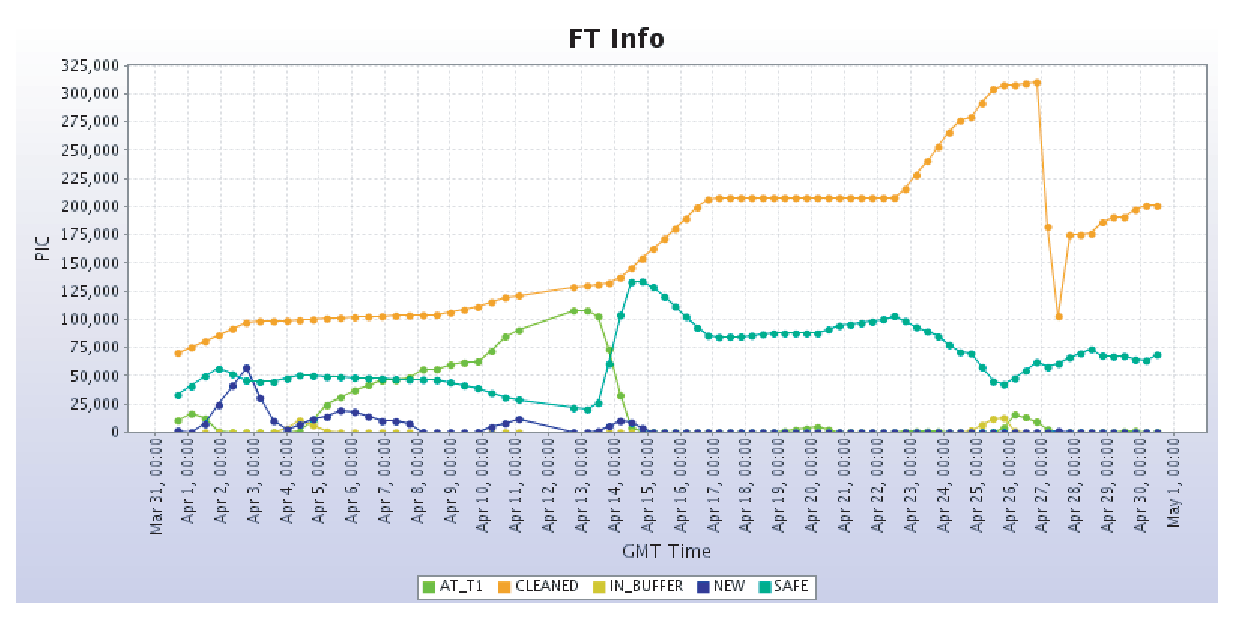
\includegraphics[width=10cm]{PIC-FT.eps}
\label{fig:PIC-FT}
\caption{Throughout DC04 the number of files apparently at the T0 and on the SE (classed as NEW or IN\_BUFFER) was negligible for PIC and CNAF (the diagram here is for PIC, but is equally applicable to CNAF), suggesting that the SE and T1 agents were able to keep up with the rate of generation of files at the T0. }
\end{figure} 

At the start of DC04 both PIC and INFN used Java RM APIs to make
transfers and catalogue lookups/registrations. This was found to be
inefficient, and both sought other methods of transfer. Interestingly,
the T1s chose subtly different methods to transfer from the T0 after
moving away from the Java API.

CNAF chose to use the Java EDG Replica Manager command line tools to
transfer and register files with some very limited use of the LRC C++
API to query the LRC for filenames to start transfers. Use of the RM
API meant that their transfers and catalogue registrations were
integral operations, and therefore more fully transactional.

PIC chose to use globus-url-copy and the LRC C++ API to register
replicas. In principle recovering from failed transfers was more
difficult for PIC, as the transfer and register operations were not
integral. This however should be weighed against CNAF's use of the
slower Java RM tools- although the use of the Java RM could be
supplanted by the use of the EDG C++ API.

Subtle variations in approach aside, transfer rates from the SE EB
could be sustained at over 2 MBps, peaking at 16 MBps
(fig. \ref{fig:SE-EB-network}), with transfer rates into CNAF and PIC
reaching a sustained 30 MBps for hours during a large-filesize stress
test at the end of DC04 (fig's. \ref{fig:PIC-stress},
\ref{fig:CNAF-stress}). Internal monitoring at CNAF revealed a
bottleneck on site, with an internal link to the SE operating at over
80\% capacity during the final stress test.

\begin{figure}[tbp]
\centering
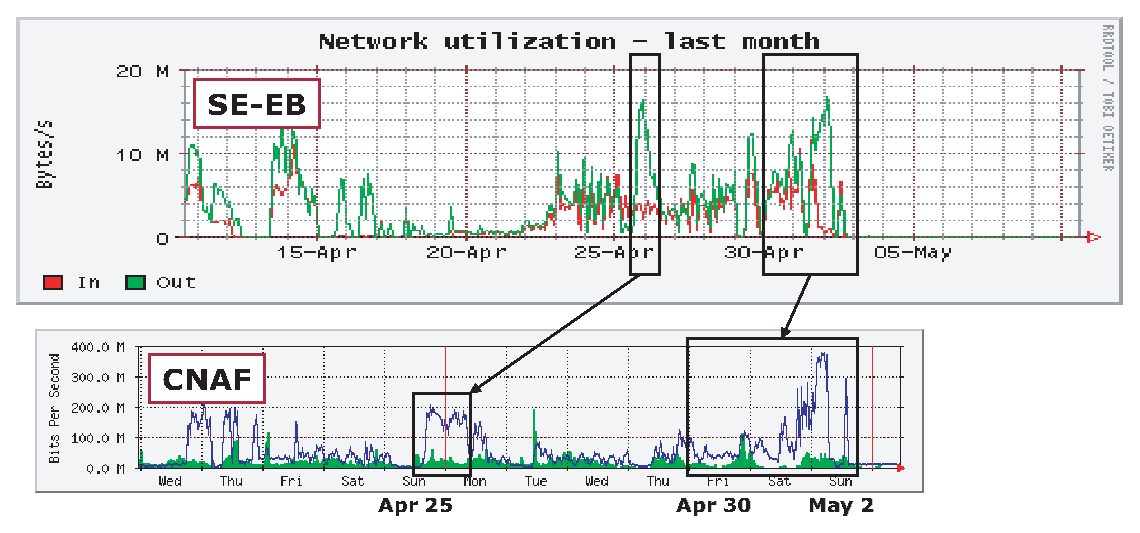
\includegraphics[width=15cm]{SE-EB-network.eps}
\label{fig:SE-EB-network}
\caption{Transfer rates out of the SE EB could be sustained at over 2 MBps toward the end of DC04, and peaked at 16MBps.}
\end{figure}

\begin{figure}[tbp]
\centering
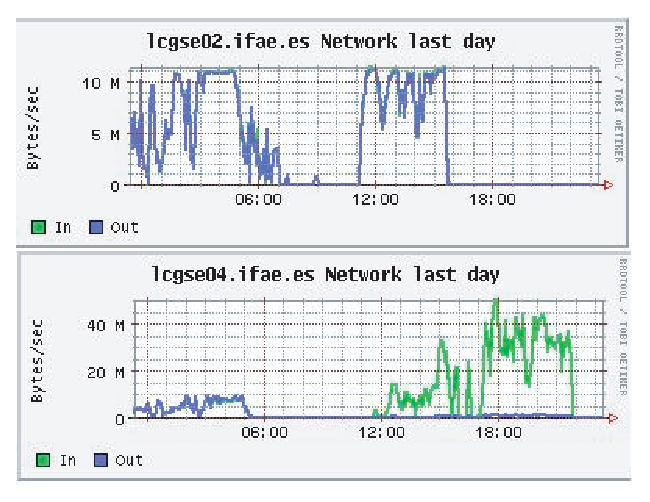
\includegraphics[width=10cm]{PIC-stress.eps}
\label{fig:PIC-stress}
\caption{During a large filesize stress test at the end of DC04, files of 600MB and larger were put into distribution. PIC sustained transfer rates of 30 MBps for 6 hours.}
\end{figure} 

\begin{figure}[tbp]
\centering
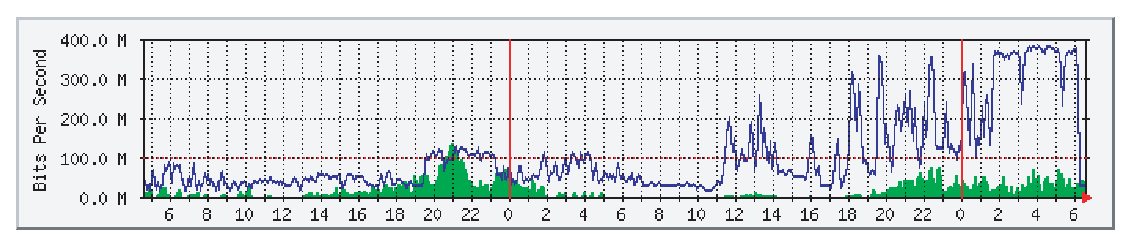
\includegraphics[width=10cm]{CNAF-stress.eps}
\label{fig:CNAF-stress}
\caption{During a large filesize stress test at the end of DC04 (the period from 0 at the right of the plot), files of 600MB and larger were put into distribution. CNAF sustained transfer rates of 40 MBps for 5 hours.}
\end{figure} 

At CNAF issues with the Castor tape stager were found to be due to the
high number of entries in its database (a consequence of the small
file size). In general tape performance was slow due to inefficient
utilization, meaning a delay in psoting files as being ``safe''. CNAF
have since been working on an import buffer and related agents to
group files more reasonably for their tape system on arrival.

In contrast PIC experienced no problems with their Castor tape.

PIC and CNAF were also able to distribute data on to T2s (CIEMAT and
Legnaro respectively) for analysis. To manage these further transfers,
as well as real-time analysis, they effetively created a new set of
distribution chains using a MySQL TMDB for collaboration information.

\section{Conclusions and future plans}
Conclusions can be drawn in three areas: organisation and coordination, distribution 
architecture, and distribution infrastructure.

\subsection{Organisation and coordination}
In general the lead-in time (the time between requirements being known
and the start of DC04) was considered too short. Despite this many
problems were tackled successfully during DC04- however, most should
have been tackled before DC04, which was eventually less about
sustained running than about establishing what needed to be done. For
DC05 however we now have a better feel for the operational issues
involved in distributing data over the WAN. T1 responsible groups
should be encouraged to have plans for providing services 6 months
before DC05, which naturally means these requirements are well
understood. A summary of operational issues should be established
between CERN and the T1s immediately.

Coordination of people invovled in agent development during DC04 was
straightforward, because the group was small and composed of actively
involved volunteers with relevant expertise in Perl, C++, Java, Oracle
and the deployment use of various middleware transfer tools. The
system description was deliberately reduced to minimal interactions
between components with well-defined responsibilities, which actively
encouraged rapid ``hacking'' and equally rapid throwing away of code
components. This approach suited the small group of experts.

Day to day running of DC04 was somewhat inefficient. Global management
of agents, and notification of local supervisors were achieved via
email. This needs to be dramatically improved in future versions of
the system. In addition, most high-output periods were scheduled for
weekends, which was not ideal, although many people involved devoted
weekend time to keeping the system running. This weekend running was
a natural by-product of the fact that development (on all aspects of
the system) tended to happen during the working week. Ideally DC05
will be more a test of deployment and tuning than ongoing development.

\subsection{Distribution architecture}
The agent system was created to fill a perceived gap in the existing
EDG and LCG Grid middleware, which had no mechanism for large-scale
(bulk) scheduling of transfers over known routes and at dataset
granularity. Middleware developers have implemented required
components and APIs, and command line tools to access those
components. Typically these were good as examples but suffered from
limited performance when used in a large scale system. From our point
of view the amount of ``grid integration'' work requried was larger
than expected.

A particular example of this was the RLS: a file catalogue is an
essential logical component of the distribution system. The RLS
supplied has no support for bulk operations, or transactional access,
and had not been tested under the load generated during DC04.  The
performance of the Java command line interface did not scale as
required (but were arguably never meant to). It should be noted that
the API proved straightforward to use, and (in part) use of the API
enabled us to meet our requirements.

It is possible that each experiment will have data scheduling
requirements unique enough that it is more efficient to define a
structure into which replica and resource management and transfer
middleware can be plugged at will. The system we have produced for
DC04 is such a generic structure, and is therefore useful input to the
ARDA/EGEE effort.

Development of the distribution scheme is likely to be coupled to very
short tiemscales as it needs to produce working systems immediately
for production use. This is a benefit as new requirements and
functionality can be quickly identified and integrated. In the short
term the development approach taken during DC04 is useful. Some long
term vision of how the system fits into some overall CMS computing
architecture is essential, however. This is particularly important for
a clean interaction between distribution and grid-based analysis,
which may also move files. Decisions such as whether distribution
seeds a ``global'' grid, or whether it seeds multiple ``national''
grids with files and handles the transfer between them have some
impact on the design of the system, and on file and site policy
regarding file priority and lifetime.

\subsection{Distribution infrastructure}
During DC04 we have identified a number of sources of throttling in
the system, and these should be investigated independently and in
detail. These throttles include access to and management of
tape/storage (at CERN and at T1s); catalogue queries and updates, and
suitability of certain catalogues for global use; use of a single
TMDB; and physical network links internal to CMS sites.

The distribution system agents require easy access to metadata- both
dedicated distribution metadata and experiment specific metadata. The
mechanism for handling most metadata was poorly developed for DC04,
and needs to be improved for future versions.

The RLS is seen as a critical bottleneck in the system. We are
currently coupled to it in three ways: transfers using the LCG RM
tools are coupled transfer-and-RLS-register operations; the analysis
jobs submitted via an LCG resource broker require an RLS for filename
lookups; and we have also triggered some intensive performance-related
development as a result of our activities, and it would be useful to
remain in touch with these. However, it is important that we
immediately consider alternative file catalogue architectures: for
example, it is possible to conceive a computing architecture in which
national (sub)grids are served by ``local'' catalogues. The RLS could
be used to store the locations of the ``local'' catalogues.

The version of SRB used during DC04 proved unable to meet the the
requirements of it: it should be noted that this is more an issue of
inadequate service provision on the part of a T1 than a problem with
SRB per se, although the problem was compounded by the use of a single
point-of-failure MCat, unaviodable in the SRB version deployed. It is
apparent that a clearer sense of ``a T1 production service'' in
relation to accepted responsibilities is required.

Logging of low level metrics- file transfer rates, etc- was handled
very well by a number of tools: MonaLISA, GridICE and Lemon. Logging
of higher level distribution system metrics was not so so well
developed. Toward the end of DC04 the number of files in each transfer
state was monitored in MonaLISA, but only for a rpedefined set of
states. In the future this needs to be extended to cover agent uptime,
transition of files through states, files handled per agent per
second, and, no doubt, others. MonaLISA is our current tool of choice
for gathering this data, and amy also provide a good global control
mechanism for agents.

\subsection{Overall conclusion}
It was shown that large scale scheduled distribution to a set of known
destinations, and subsequent analysis, was possible at 25Hz, or with a
20 minute turnaround time, or at very high transfer rates. This gives
us confidence that future versions will be able to handle this load
consistently, and for sustained periods. The variability in
performance between different agent deployments shows that there is
some exploratory work to be done in determining best practice for
deployment and use.

\bibliographystyle{plain}
\bibliography{dc04-post-mortem}

\end{document}